% (The MIT License)
%
% Copyright (c) 2023-2024 Yegor Bugayenko
%
% Permission is hereby granted, free of charge, to any person obtaining a copy
% of this software and associated documentation files (the 'Software'), to deal
% in the Software without restriction, including without limitation the rights
% to use, copy, modify, merge, publish, distribute, sublicense, and/or sell
% copies of the Software, and to permit persons to whom the Software is
% furnished to do so, subject to the following conditions:
%
% The above copyright notice and this permission notice shall be included in all
% copies or substantial portions of the Software.
%
% THE SOFTWARE IS PROVIDED 'AS IS', WITHOUT WARRANTY OF ANY KIND, EXPRESS OR
% IMPLIED, INCLUDING BUT NOT LIMITED TO THE WARRANTIES OF MERCHANTABILITY,
% FITNESS FOR A PARTICULAR PURPOSE AND NONINFRINGEMENT. IN NO EVENT SHALL THE
% AUTHORS OR COPYRIGHT HOLDERS BE LIABLE FOR ANY CLAIM, DAMAGES OR OTHER
% LIABILITY, WHETHER IN AN ACTION OF CONTRACT, TORT OR OTHERWISE, ARISING FROM,
% OUT OF OR IN CONNECTION WITH THE SOFTWARE OR THE USE OR OTHER DEALINGS IN THE
% SOFTWARE.

\documentclass{article}
\usepackage{../sqm}
\newcommand*\thetitle{Tech Debt}
\begin{document}

\plush{\sqmTitlePage{14}{pvZDcytPU3w}}

\qte
  [Ward Cunningham]
  {../05-maintainability-index/ward-cunningham.jpg}
  {Shipping first time code is like going into \ul{debt}. A little debt speeds development so long as it is paid back promptly with a rewrite. The danger occurs when the debt is not repaid. Every minute spent on not-quite-right code counts as \ul{interest} on that debt.}
  {cunningham1992}

\pptBanner{Puzzle Driven Development: Motivating Example}
\begin{pptWide}{3}
Commit \#1:\par
{\scriptsize\begin{ffcode}
int fibonacci(int n) {
  if (n <= 2) {
    return 1;
  }
  (*@\textcolor{orange}{// @todo I don't know}@*)
  (*@\textcolor{orange}{// what to do when "n"}@*)
  (*@\textcolor{orange}{// is larger than "2".}@*)
  (*@\textcolor{orange}{// Implement it and uncomment}@*)
  (*@\textcolor{orange}{// the assertion below.}@*)
  return 0;
}
assert fibonacci(0) == 1;
assert fibonacci(2) == 1;
(*@\textcolor{orange}{// assert fibonacci(9) == 34;}@*)
\end{ffcode}
}
\par\columnbreak\par
Commit \#2:\par
{\scriptsize\begin{ffcode}
int fibonacci(int n) {
  if (n <= 2) {
    return 1;
  }
  if (n == 9) {
    return 34;
  }
  (*@\textcolor{orange}{// @todo Implement others}@*)
  (*@\textcolor{orange}{// too, but I don't know}@*)
  (*@\textcolor{orange}{// how to do it right.}@*)
  return 0;
}
assert fibonacci(2) == 1;
assert fibonacci(9) == 34;
(*@\textcolor{orange}{// assert fibonacci(10) == 55;}@*)
\end{ffcode*}
}
\par\columnbreak\par
Commit \#3:\par
{\scriptsize\begin{ffcode}
int fibonacci(int n) {
  if (n <= 2) {
    return 1;
  }
  return fibonacci(n-1)
    + fibonacci(n-2);
}
assert fibonacci(0) == 1;
assert fibonacci(2) == 1;
assert fibonacci(9) == 34;
assert fibonacci(10) == 55;
\end{ffcode}
}
\end{pptWide}
\plush{}

\plush{
\pptBanner{Break-and-Fix Cycle}
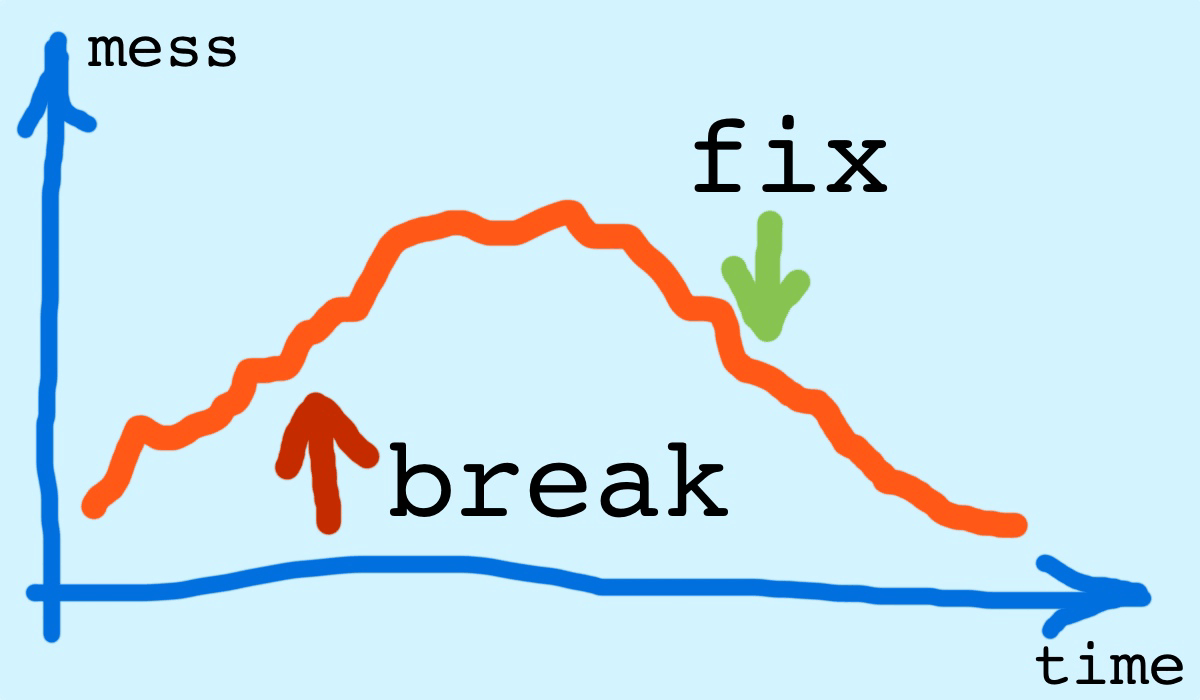
\includegraphics[width=.7\textwidth]{time-and-mess-diagram.png}\par
{\scriptsize Source: \url{https://www.yegor256.com/2014/04/12/puzzle-driven-development-by-roles.html}\par}}

\plush{
\pptBanner{\texttt{www.0pdd.com}}
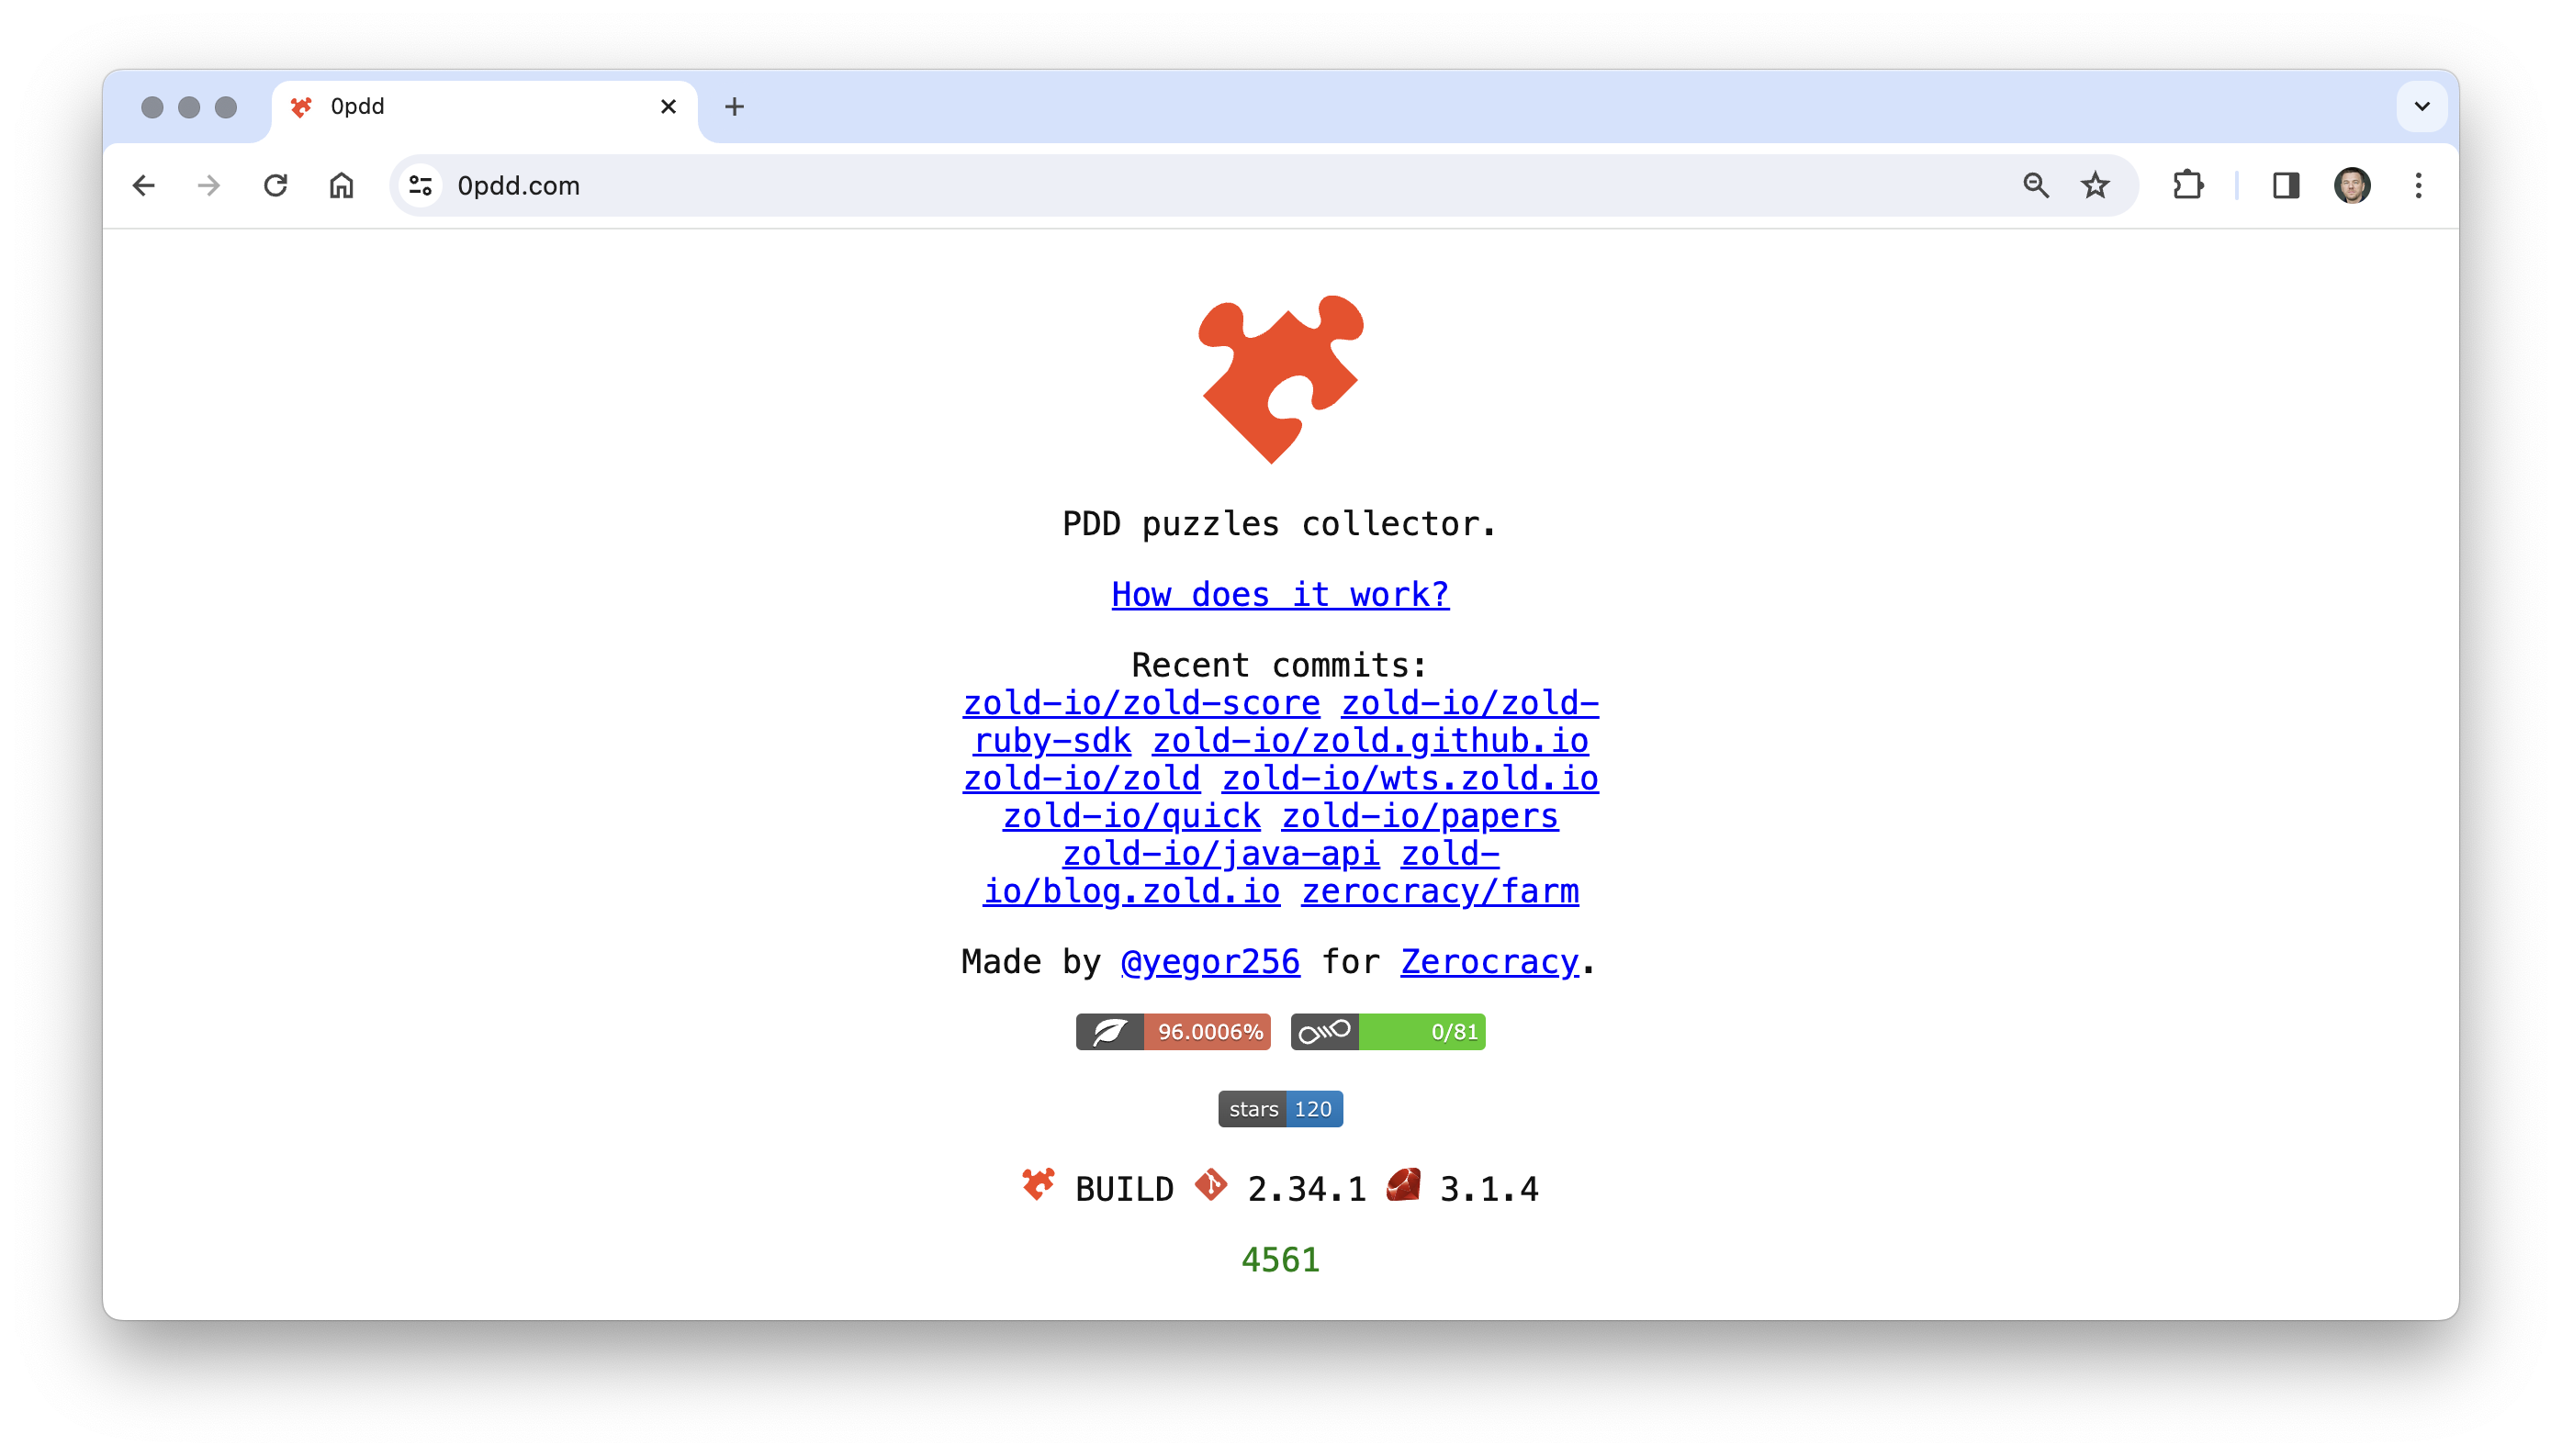
\includegraphics[width=.8\textwidth]{0pdd-front.png}}

\plush{\pptBanner{PDD Pipeline}
\begin{tikzpicture}[node distance=6em, every edge/.style={line width=.1em, draw, ->}, every node/.style={fill=white}]
\tikzstyle{actor} = [draw, line width=.1em,font={\Large},outer sep=.2em]
\node[actor] (coder1) {Coder \#1};
\node[actor,right=of coder1] (git) {Git};
\node[actor,right=of git] (0pdd) {0pdd.com};
\node[actor,below=of 0pdd] (tts) {TTS};
\node[actor,left=of tts] (coder2) {Coder \#2};
\path (coder1) edge node {push} (git);
\path (git) edge[bend left=30] node {webhook} (0pdd);
\path (0pdd) edge[bend left=30] node {submit ticket} (tts);
\path (coder2) edge[bend right=30] node {self-assign} (tts);
\path (coder2) edge[dashed] (git);
\end{tikzpicture}}

\plush{
\pptBanner{250+ Puzzles in \texttt{objectionary/eo}}
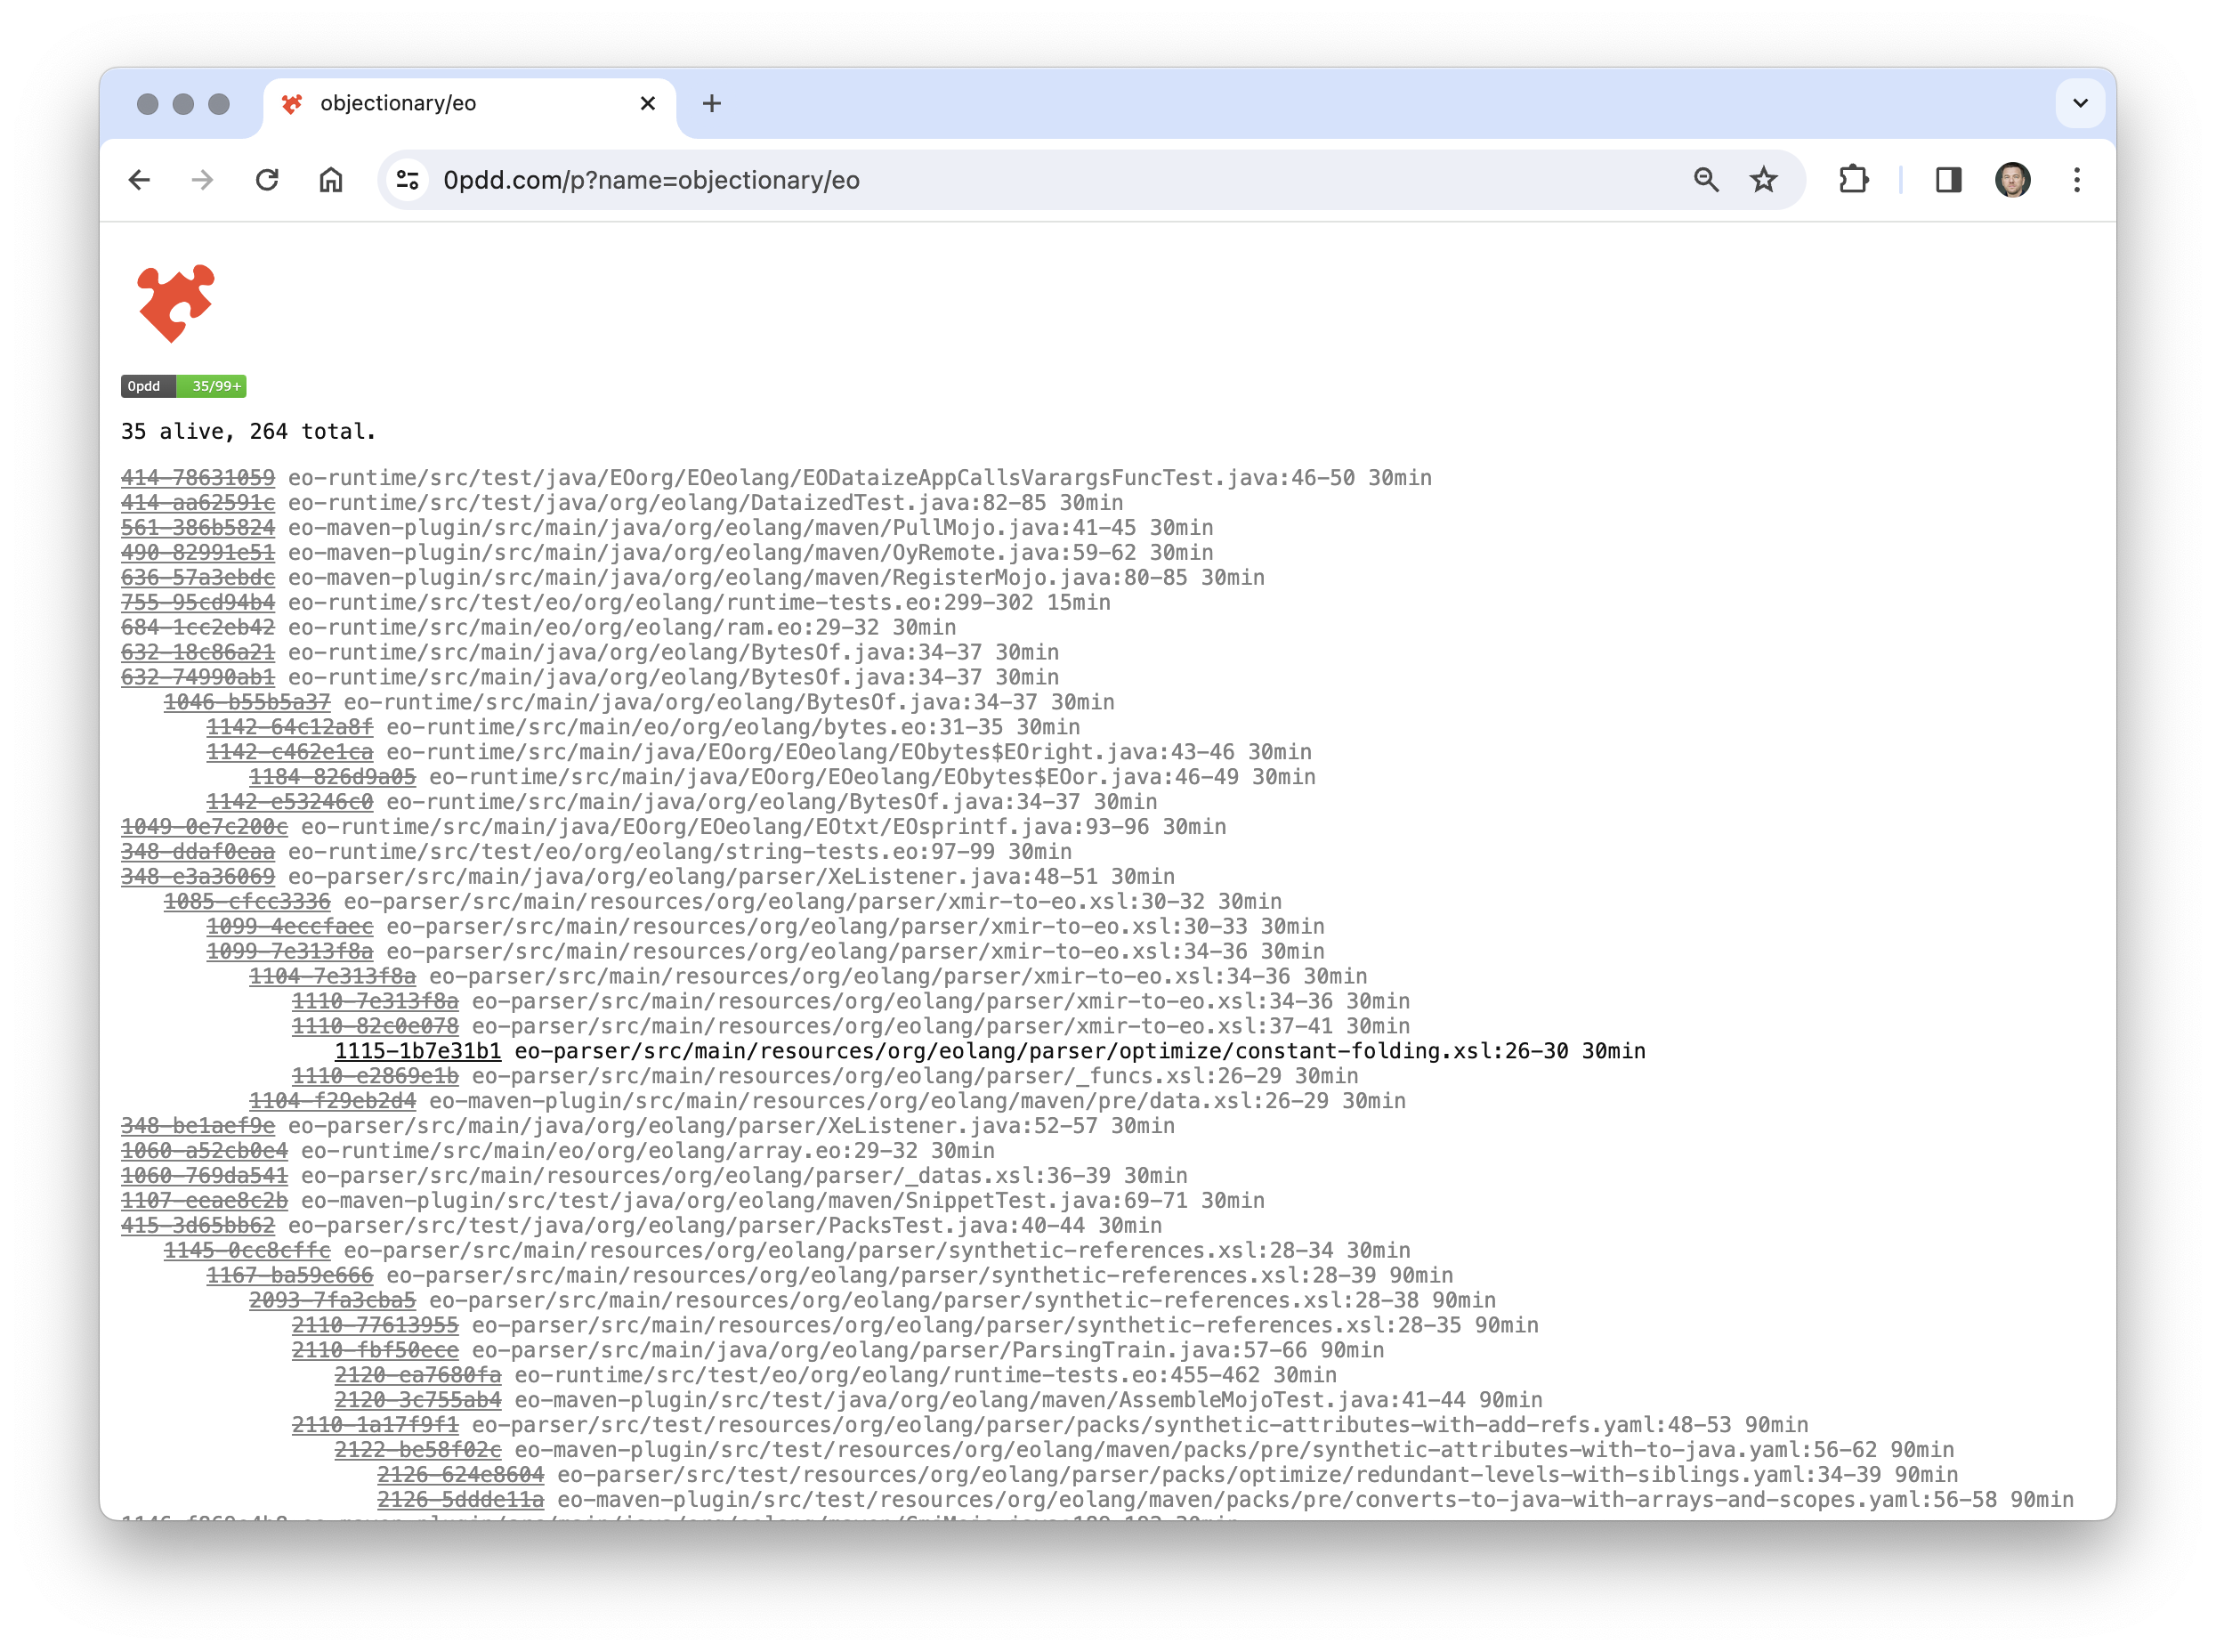
\includegraphics[width=.6\textwidth]{0pdd-screenshot.png}\par
{\small Source: \url{https://www.0pdd.com/p?name=objectionary/eo}\par}}

\plush{
\pptBanner{Sample Ticket Submitted by 0pdd.com to \texttt{objectionary/eo}}
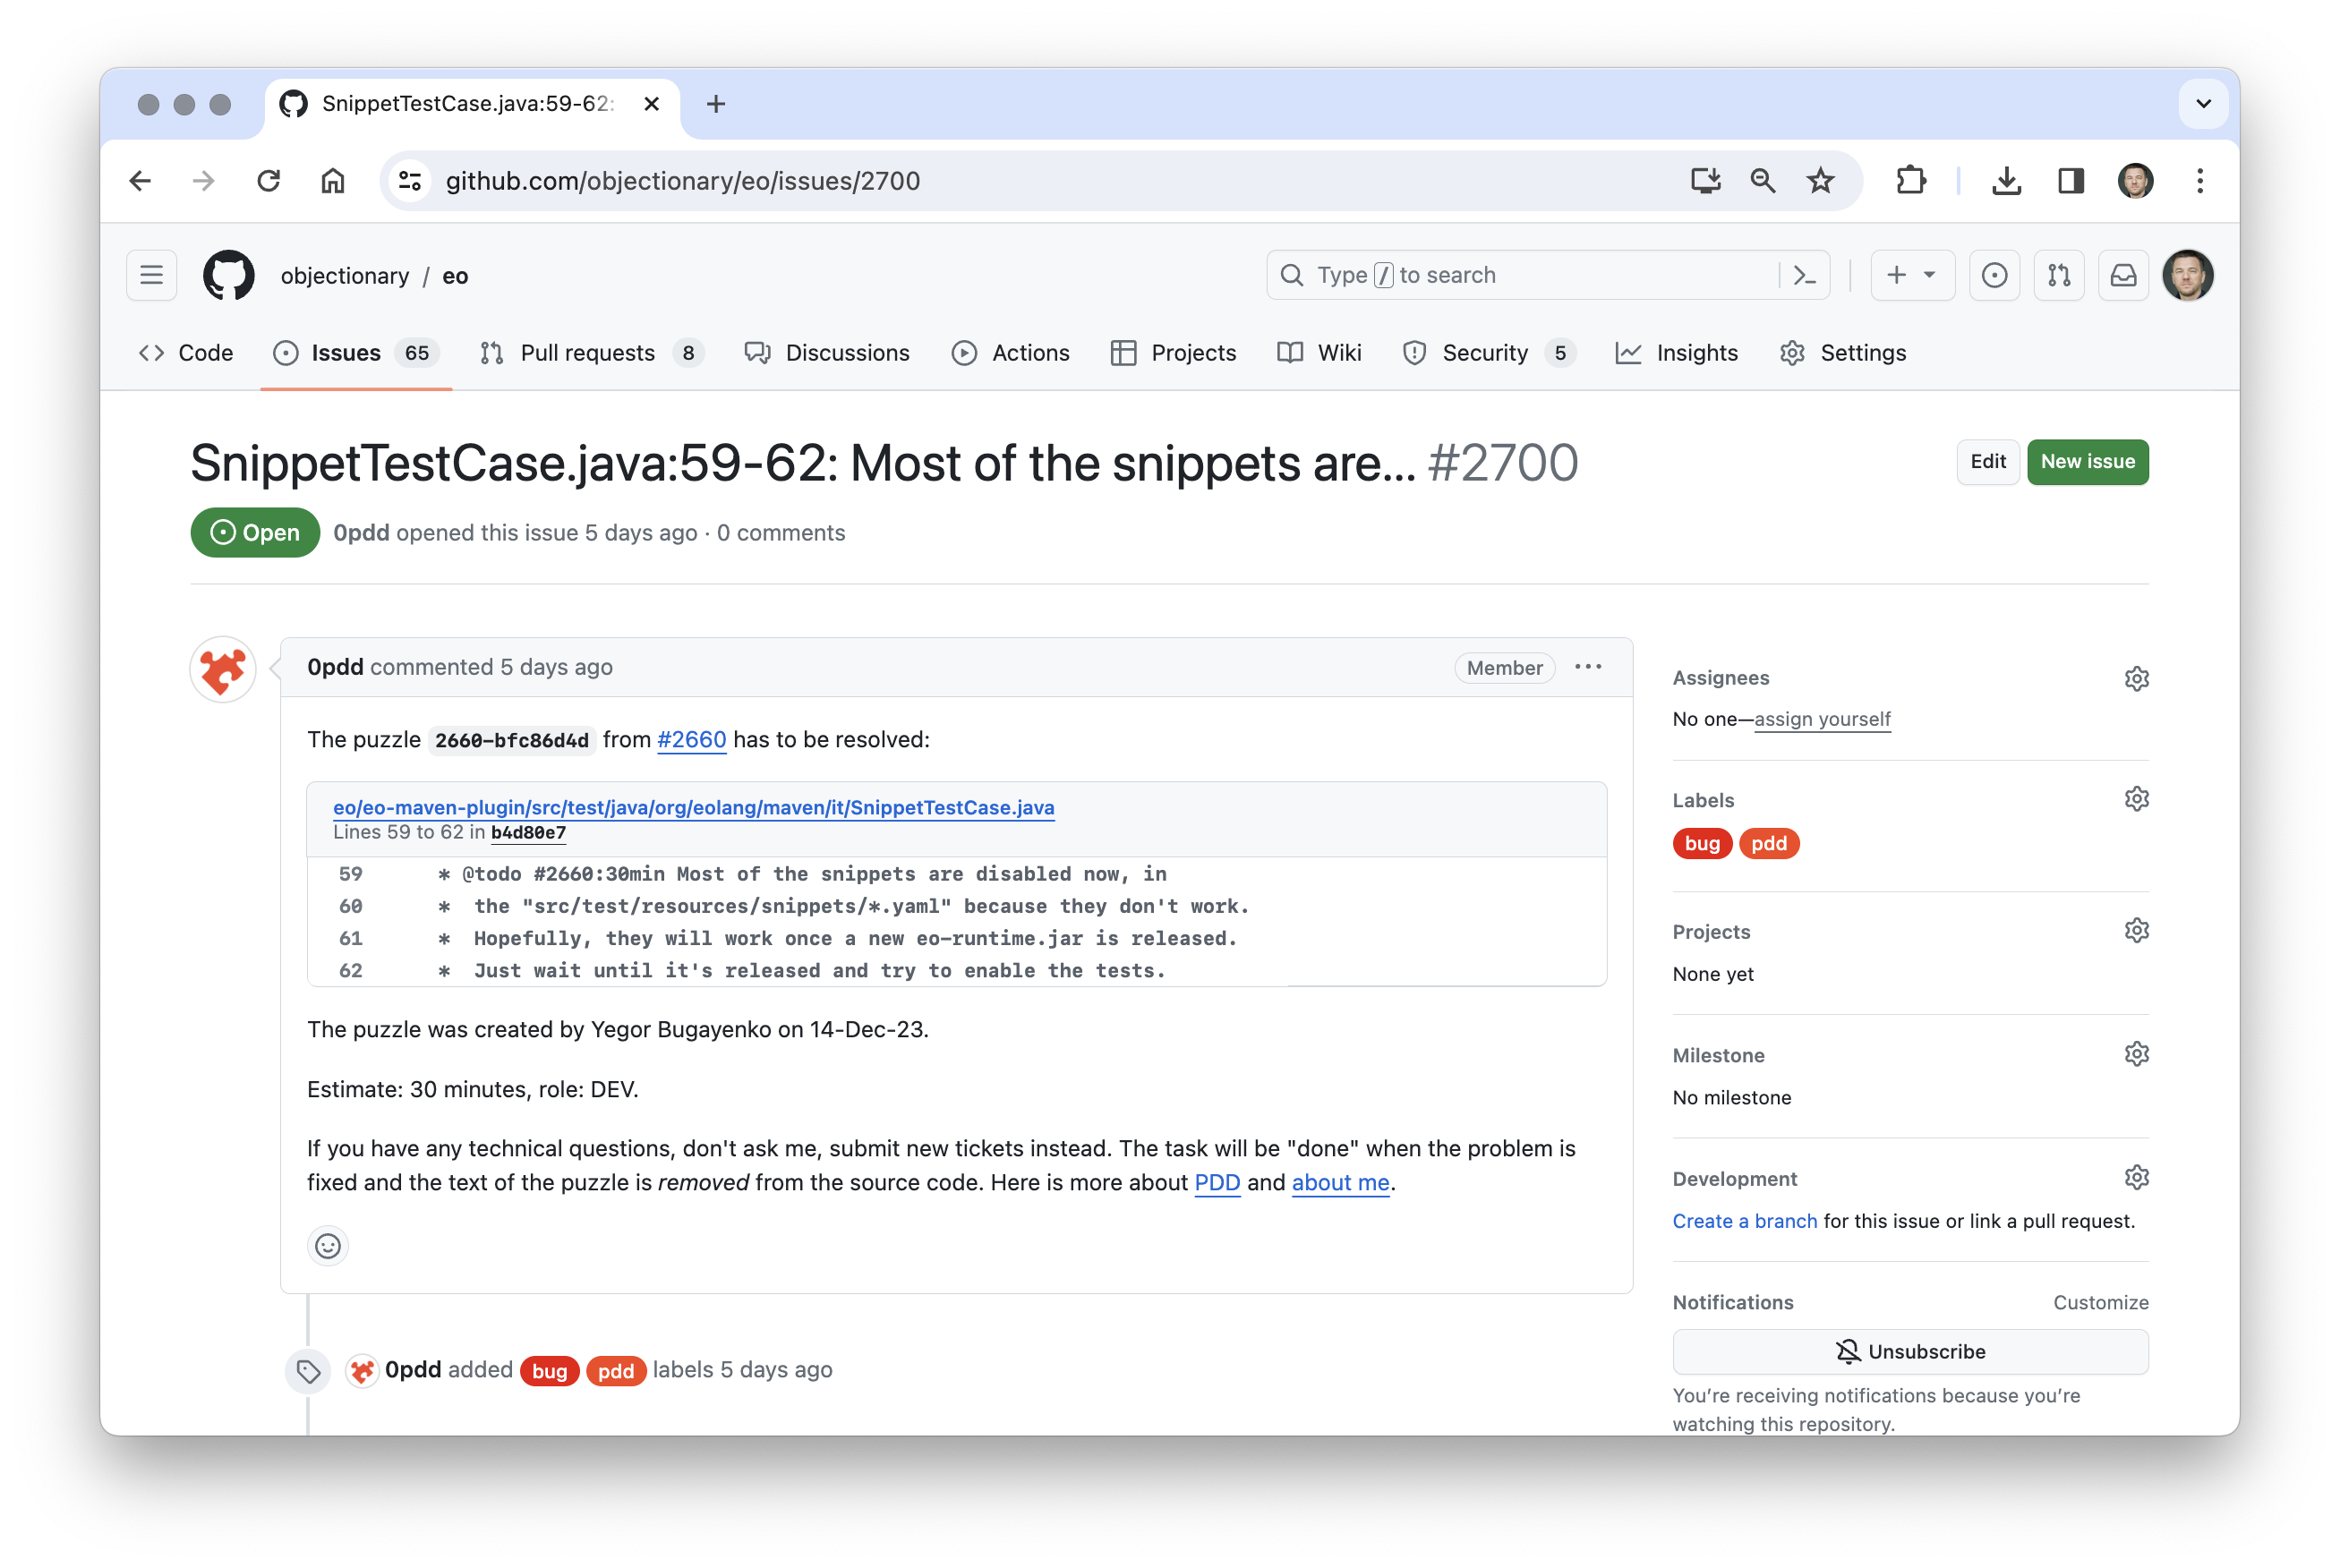
\includegraphics[width=.6\textwidth]{ticket.png}\par
{\small Source: \url{https://github.com/objectionary/eo/issues/2700}\par}}

\qte
  [Yegor Bugayenko, Mirko Farina, Artem Kruglov, Witold Pedrycz, Yaroslav Plaksin, \ul{Giancarlo Succi}]
  {giancarlo-succi.jpg}
  {This paper presents the benefits of considering the entire backlog when prioritizing tasks. We employ an iterative approach using Particle Swarm Optimization to optimize a linear model with various preprocessing methods to determine the optimal model
for task prioritization within a backlog.}
  {bugayenko2023}

\plush{
  \pptBanner{Read this:}\par
  \small
  \textit{Automatically Prioritizing and Assigning Tasks from Code Repositories in Puzzle Driven Development},
    Yegor Bugayenko, Ayomide Bakare, Arina Cheverda, Mirko Farina, Artem Kruglov, Yaroslav Plaksin, Giancarlo Succi, and Witold Pedrycz,
    Proceedings of the International Mining Software Repositories (MSR), 2022\par
  \textit{Automatically Prioritizing Tasks in Software Development},
    Yegor Bugayenko, Mirko Farina, Artem Kruglov, Witold Pedrycz, Yaroslav Plaksin, and Giancarlo Succi,
    IEEE Access, Vol.~11, 2023 \par
  \href{https://www.yegor256.com/2010/03/04/pdd.html}{Puzzle Driven Development} (2010) \par
  \href{https://www.yegor256.com/2014/04/12/puzzle-driven-development-by-roles.html}{PDD by Roles} (2014) \par
  \href{https://www.yegor256.com/2017/04/05/pdd-in-action.html}{PDD in Action} (2017) \par
}

\end{document}
